\subsection{Corpi minori del sistema solare}

\begin{frame}{Corpi minori: origine ed evoluzione.}
\begin{itemize}
\item MB: \num{e5} asteroids, $M_{T}\approx\num{5e-4}\mearth{}$: less mass than expected from smooth distribution in primordial nebula.
\item Why there is so little mass remaining in asteroid region ($\approx\SI{3}{\astronomicalunit}$)? 
\item Why is this mass spread over so many body??
\item Why most of asteroid orbits are more inclinated/eccentric than that of major planets?
\item Why are asteroid so compositionally diverse?
\item Satelliti e anelli
\item Kuiper Belt require that planetesimal exist beyond Neptune; Why the abrupt cut-oof beyond Neptune?
\item Oort cloud: Mass of solid material eject from planetary (giants) region \numrange{1}{1000}$\mearth{}$
\end{itemize}
\end{frame}

\begin{wordonframe}{Asteroidi, comete, TNO, ogetti della fascia di Kuiper-Edgeworth.}
In asteroid regions there is 2-3 order of magnitude less mass than expected from smooth mass distribution in primordial nebula.

Orbital resonances can also destabilize one of the orbits. For small bodies, destabilization is actually far more likely.

Secular resonances: mean drift of pericentre becomes commensurable with one of proper frequency of planetary system

In the asteroid belt beyond 3.5 AU from the Sun, the 3:2, 4:3 and 1:1 resonances with Jupiter are populated by clumps of asteroids (the Hilda family, the few Thule asteroids, and the extremely numerous Trojan asteroids, respectively).
\end{wordonframe}

\subsection{Asteroidi. Main Belt.}\linkdest{asteroids}

\begin{frame}{Caratteristiche main belt}
\begin{columns}[T]\begin{column}{0.5\textwidth}
\begin{block}{Classificazione fotometrica}
\begin{itemize}
    \item C: Condriti carbonacee. Low albedo, flat spectrum in V-NIR.
    \item S: high albedo, silicates absorption band
    \item D-type: very red (low temperature, organic compounds: $CH_4$, etc)
    \item M-type: $A\approx0.1$, reddish
\end{itemize}
\end{block}
\end{column}\begin{column}{0.5\textwidth}
\begin{figure}[!ht]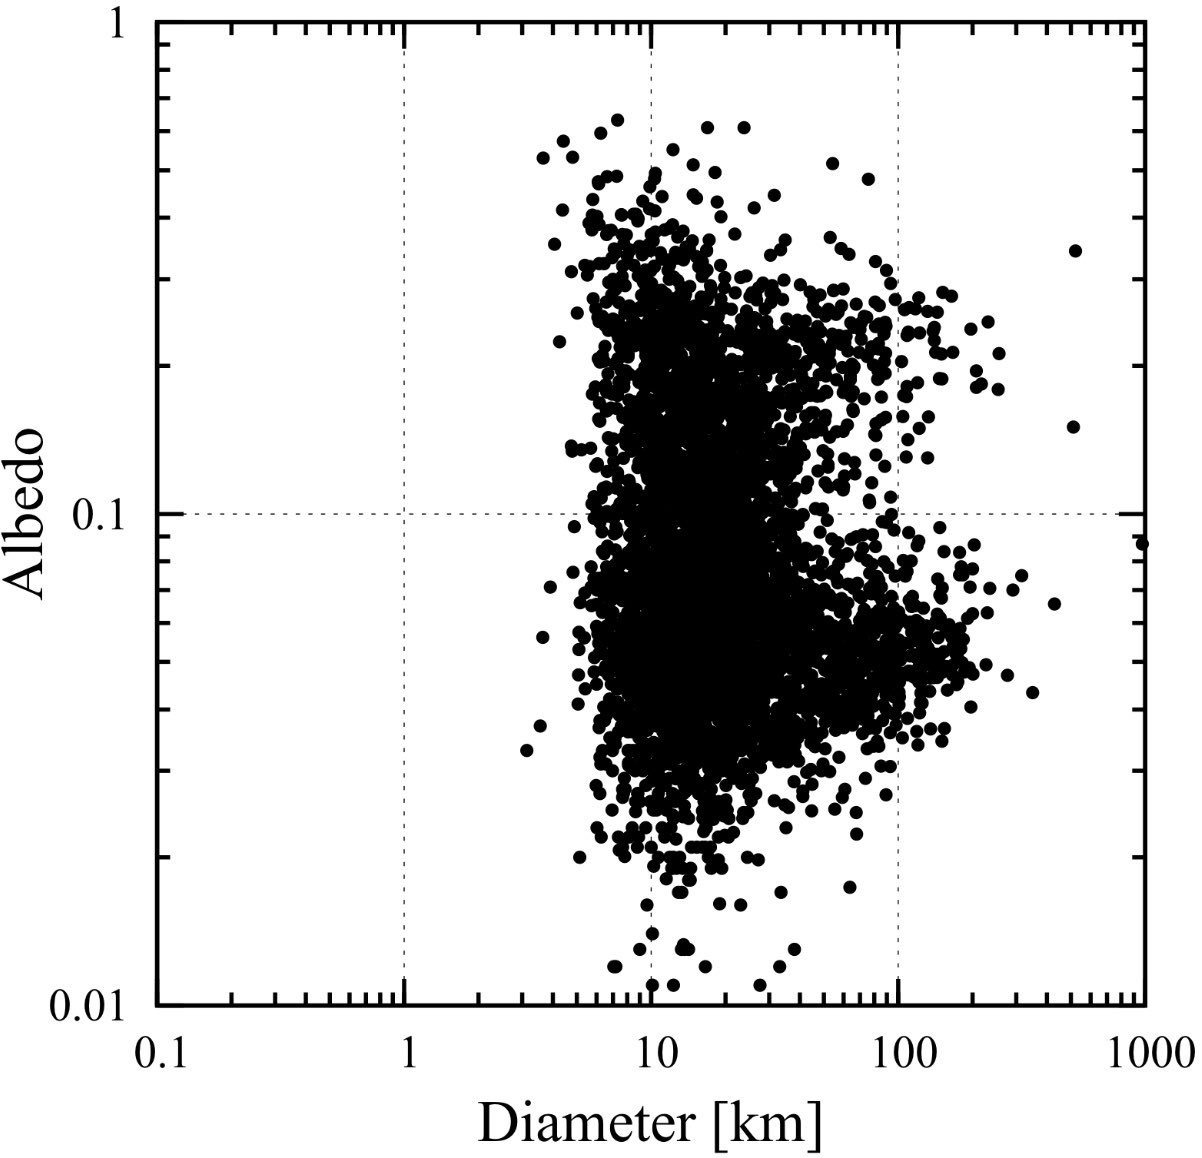
\includegraphics[keepaspectratio,angle=-90,origin=c,width=0.95\textwidth]{A-D}\end{figure}
\begin{block}{Composizione}
Absorption band: silicates, water ices, hydrated minerals.
\end{block}
\end{column} \end{columns}
\begin{block}{Classificazione dinamica}
\begin{itemize}
\item Fascia principale: tra Marte (perielio \SI{1.66}{\astronomicalunit}) e Giove.
\item Rapido spopolamento man mano che ci si avvicina a Giove.
\item Lacune di Kirkwood: per valori del semi-asse maggiore risonanti con quello di Giove.
\item grouping of proper elements: famiglie collisionali
\item Evolution $\tau\si{\mega\year}$: increasing eccentricity cause collision with inner planets or Sun
\end{itemize}
\end{block}
\end{frame}

\begin{wordonframe}{Classificazione asteroidi: orbita, spin, albedo, etc}
Sono la principale sorgente di meteoriti.
Orbite comprese tra Marte e Giove. Il primo \'e 1Ceres, diametro circa \SI{1000}{\kilo\meter}.
Da Terra si vedono come sorgenti puntiformi. Forma, dimensioni e caratteristiche superficiali: tecniche interferometriche e fenomeni di occultamento.
La spettro di riflessione \'e vario: dipende dalle caratteristiche chimiche e fisiche della superficie.
(hydrated minerals includes $H_2O$, $OH$ in crystall structure)
Paucity of asteroid in mean motion/secular resonance with planets.
Disruptive collisions (mean $v_r$ circa 4 $v_e$(ceres)$\approx\SI{5}{\kilo\meter\per\second}$).
Large metallic asteroids: differentiated primordial object stripped of their mantle.
\end{wordonframe}

\begin{frame}{Evoluzione. Kirkwood gap: Resonances in main belt}
\begin{figure}[!ht]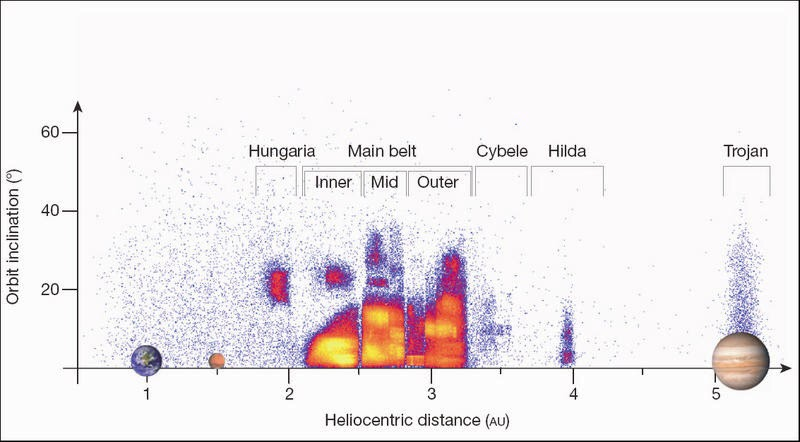
\includegraphics[keepaspectratio,width=0.9\textwidth]{MBplanets}
\end{figure}
\begin{block}{Perturbation}
\begin{itemize}
\item Collisioni: disruptive collisions (truncation at Mars perihelion \SI{1.66}{\astronomicalunit}), inject in resonannt regions, A. families,
\item Resonances: ejection solar system, NEO.
\item Proper elements excitation ($\tau\approx\SIrange{10}{50}{\mega\year}$): $\bar{e}\approx0.13$, $\bar{I}\approx\ang{7}$.
\end{itemize}
\end{block}
\begin{block}{Resonances}
\begin{itemize}
\item 3/1 mean motion resonance with Jupiter (\SI{2.5}{\astronomicalunit}) is instable due to secular resonance: eccentricity increse close to 1 due to collision or Yarkovsky effect
\item First order resonance 2/1, 3/2, 4/3 with J stable: (Z), (H), (T).
\item $\nu_6$ longitude of pericentre drift $\varpi$ drift due to Jupiter perturbation at rate $g_6\approx\SI{28.2}{\arcsecond\per\year}$: truncation at \SI{2.1}{\astronomicalunit} and bent in $(a,I)$ plane.
\end{itemize}
\end{block}
\end{frame}

\begin{wordonframe}{resonances in MB (distribuire)}

$\varpi=\Omega+\omega$: (longitudine del nodo ascendente e argomento del periastro).

In the asteroid belt within 3.5 AU from the Sun, the major mean-motion resonances with Jupiter are locations of gaps in the asteroid distribution, the Kirkwood gaps (most notably at the $3:1$, $5:2$, $7:3$ and $2:1$ resonances).

The perihelion secular resonance between asteroids and Saturn  helps shape the asteroid belt. Asteroids which approach it have their eccentricity slowly increased until they become Mars-crossers, at which point they are usually ejected from the asteroid belt by a close pass to Mars. This resonance forms the inner and "side" boundaries of the asteroid belt around 2 AU, and at inclinations of about $\ang{20}$.

Asteroids have been ejected from these almost empty lanes by repeated perturbations. However, there are still populations of asteroids temporarily present in or near these resonances. For example, asteroids of the Alinda family are in or close to the $3:1$ resonance, with their orbital eccentricity steadily increased by interactions with Jupiter until they eventually have a close encounter with an inner planet that ejects them from the resonance.

A secular resonance occurs when the precession of two orbits is synchronised (usually a precession of the perihelion or ascending node). A small body in secular resonance with a much larger one (e.g. a planet) will precess at the same rate as the large body. Over long times (a million years, or so) a secular resonance will change the eccentricity and inclination of the small body.
\end{wordonframe}

\begin{frame}{famiglie collisionali: grouping in space of proper elements}
\begin{columns}[T]
\begin{column}{0.65\textwidth}
\begin{figure}[!ht]
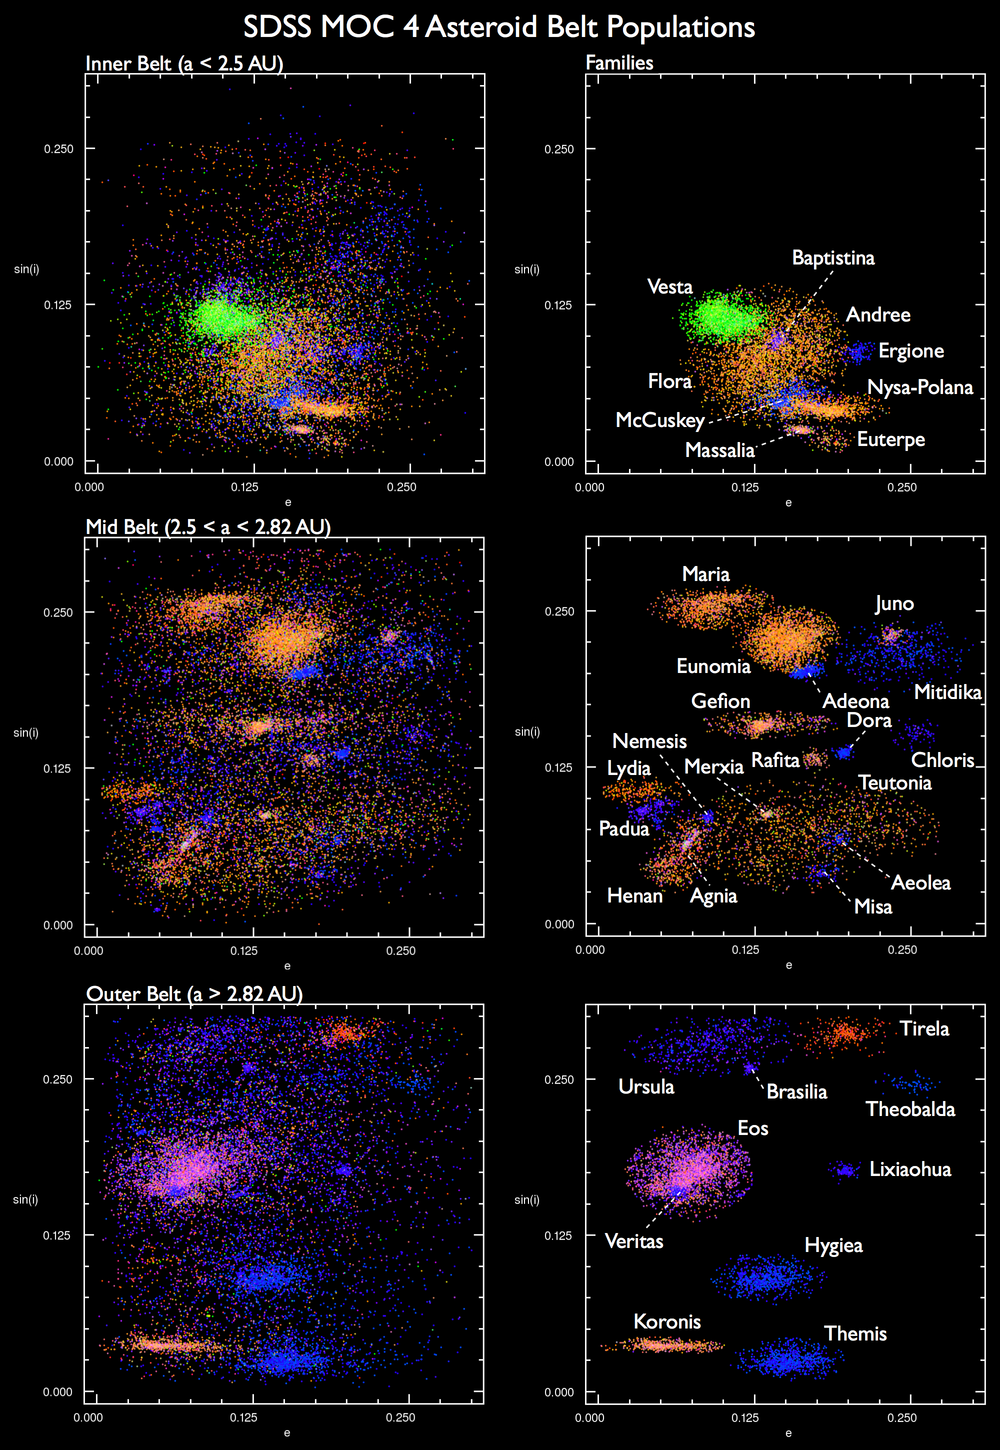
\includegraphics[keepaspectratio,height=0.85\textheight]{Asdss}
\end{figure}
\end{column}
\begin{column}{0.35\textwidth}
Collisional breakup of parent body (Hirayama): velocit\'a relative dei frammenti risultanti molto minori della velocit\'a orbitale.
\begin{block}{Families formation (dynamical aging)}
\begin{itemize}\item Entiere disruption of A. by similar size projectile \item Ejecta from non disruptive collisions (Vesta)
\item oggetti pi\'u grandi sono pi\'u rappresentativi della popolazione iniziale
\end{itemize}
\end{block}
\end{column}
\end{columns}
\end{frame}

\begin{wordonframe}{famiglie collisionali}\tolbf
\begin{block}{Distruptive collisione}
Velocit\'a relativa media \SI{5}{\kilo\meter\per\second} (4 times $v_e$(Ceres))
\end{block}
Most pop. families (similar surface composition): Themis, EOS, Koronis, Vesta. Age: \SIrange{1}{3}{\giga\year}.
\end{wordonframe}

\begin{frame}{Distribuzione di massa degli asteroidi: legge di potenza.}
\begin{block}{Collisional cascade}
\begin{columns}[T]\begin{column}{0.5\textwidth}
Popolazione di asteroidi $N_1$, $N_2$ con $m_1\gg m_2$.
Stato stazionario: $N_1=\gamma N_2$.
\end{column}\begin{column}{0.5\textwidth}
\begin{align*}
&\TDy{t}{N_1}=-\alpha\sigma_1N_1^2\\
&\TDy{t}{N_2}=(-\frac{N_2}{\tau})-\alpha\sigma_2N_1^2+(\frac{m_1}{m_2})\alpha\sigma_1N_1^2
\end{align*}
Sezioni d'urto geometriche: $\sigma_1=\sigma_2(\frac{m_1}{m_2})\expy{\frac{2}{3}}$.
\begin{equation*}
N_2=(\frac{m_1}{m_2})\expy{\frac{5}{6}}N_1
\end{equation*}
\end{column}  \end{columns}
\end{block}
\begin{block}{Legge di potenza alla Dohnanyi}
 Numero di oggetti in $[m,m+dm]$
\begin{equation*}
n(m)\propto m\expy{-\frac{11}{6}}
\end{equation*}
\end{block}
\begin{block}{$\alpha$ osservato}
MB: $\alpha\approx\numrange{1.3}{2}$
Lab.: $\alpha\approx1.8$
Large bodies ($D>\SI{10}{\kilo\meter}$): $\alpha\approx2.1$
NEO: $\alpha\approx1.58$
\end{block}
\end{frame}

\begin{wordonframe}{Distro massa A: legge di potenza.}
\begin{block}{Collisional cascade (Dohnanyi 1969) semplificata}
\begin{itemize}
\item Popolazioni stazionarie
\item Evoluzione collisionale: $\sigma\approx r^2$.
\item scaling ideale: effetto di collisione dipende dai rapporti di massa
\end{itemize}
Popolazione di asteroidi $N_1$, $N_2$ con $m_1\gg m_2$: asteroidi grandi spopolati da collisioni i cui frammenti popolano $N_2$, inoltre $N_2$ sono spopolati da collisioni e processo dinamico ($\tau$).
Stato stazionario: $N_1=\gamma N_2$, se $q=\frac{m_2}{m_1}\ll1$ $\gamma=-\frac{q}{2}+\sqrt{(\frac{q}{2})^2+q\expy{\frac{5}{3}}}$.
\end{block}
\end{wordonframe}

\begin{frame}{Size distribution}
\begin{block}{Size distro}
\begin{figure}[!ht]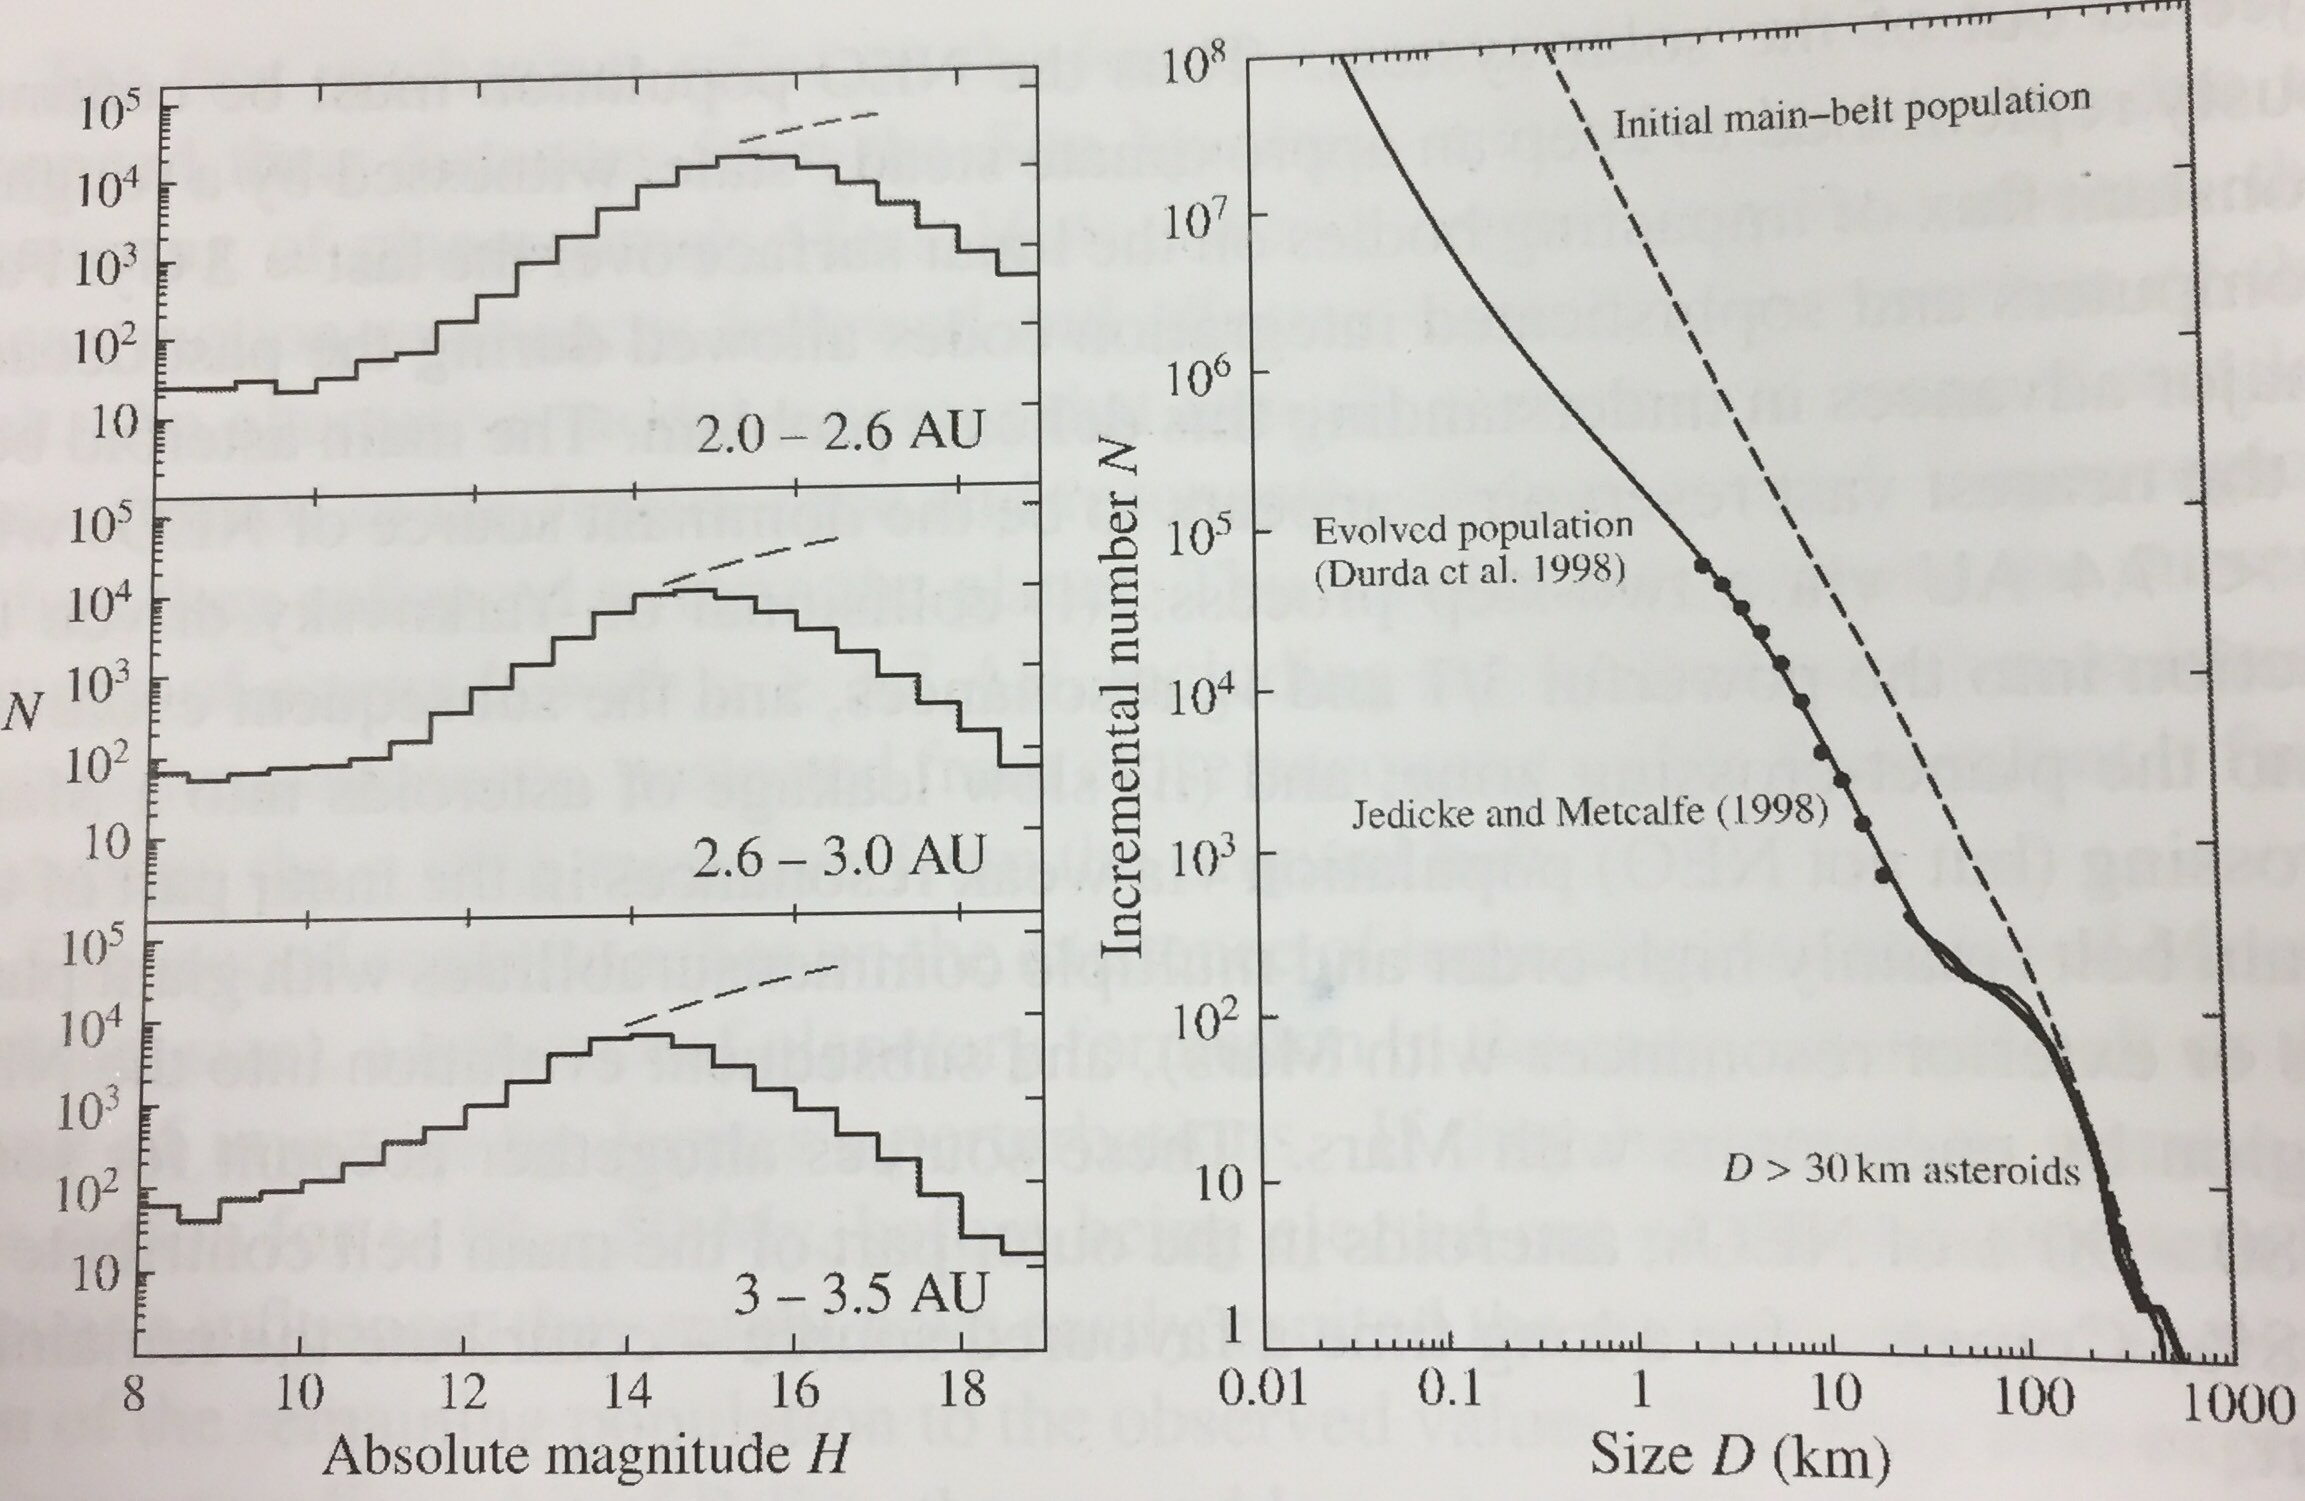
\includegraphics[keepaspectratio,width=\textwidth]{Asizedistro}
\end{figure}
\end{block}
\end{frame}

\begin{wordonframe}{Distribuzione di massa A.}
Most of A mass lies in largest bodies. Excess of bodies around \SI{100}{\kilo\meter}: self-gravitation becomes important at this size for reaccumulation
Distribuzione alla Dohnanyi  $dN\propto m\expy{-\alpha}\,dm\propto D\expy{\beta}\,dD$ (MB:$q<2$)
\end{wordonframe}

\begin{frame}{Depletion of primordial MB}
\begin{columns}[T]\begin{column}{0.5\textwidth}
\begin{itemize}
\item Sweeping mean motion resonances with Jupiter
\item Scattering action of massive planetesimal: left-over of planetary formation or injection by Jupiter perturbation.
\end{itemize}
\end{column}\begin{column}{0.5\textwidth}
\begin{itemize}
\item Effects due to Saturn/Jupiter migration
\item Cluster of core in Jupiter region: depletion of region with $a>\SI{3.3}{\astronomicalunit}$
\end{itemize}
\end{column}\end{columns}
\end{frame}

\begin{frame}{Spin rate}
\begin{columns}[T]
\begin{column}{0.5\textwidth}
\begin{figure}[!ht]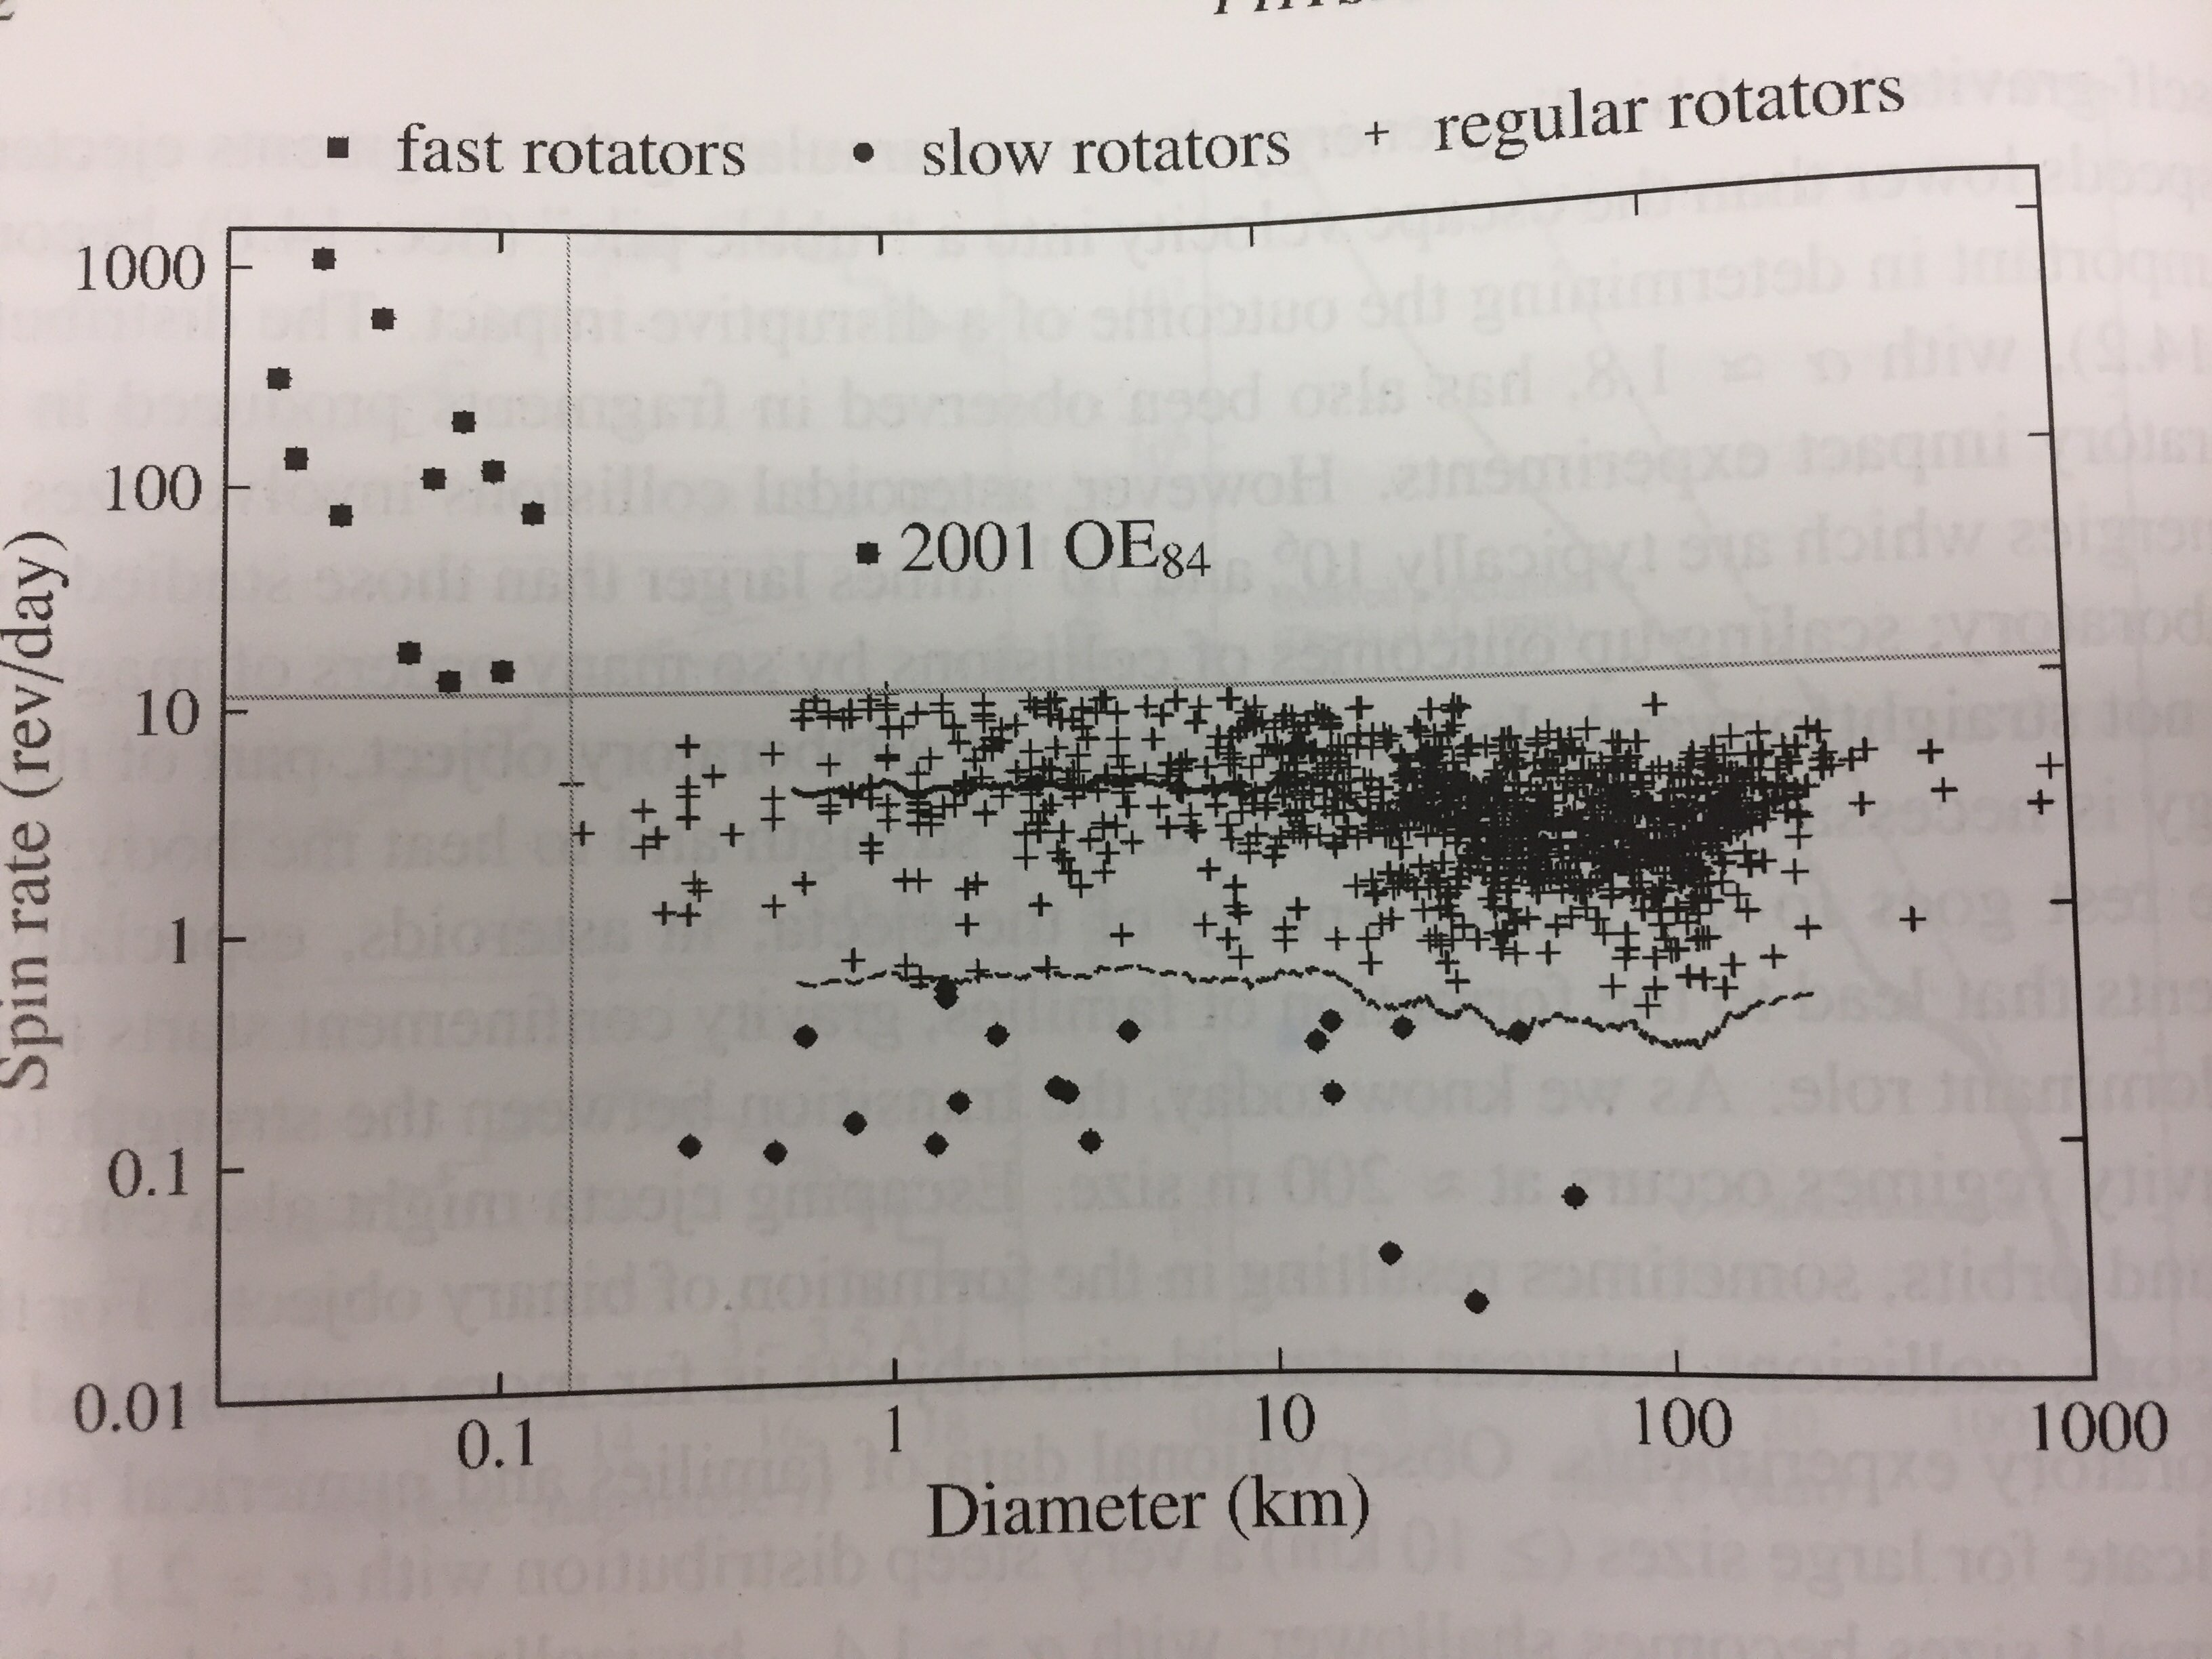
\includegraphics[keepaspectratio,width=0.99\textwidth]{spinD}
\end{figure}
Angular momentum changed by collision and dynamical processes.
\end{column}
\begin{column}{0.5\textwidth}
\begin{itemize}
\item Slow/Fast rotator: $\omega_{cr}\approx\SI{2.1}{\hour}$ (vanishing strength, $\bar{\rho}=\SI{2.5}{\gram\per\cubic\cm}$).
\end{itemize}
\begin{block}{Slow rotator}
Braking: loss of close satellite, radiation torque (smaller)
\end{block}
\begin{block}{Binary Asteroid}
\begin{itemize}\item $20\%$ NEO
\item Small eccentricity of rel. motion
\item Formation: tidal fission, capture of ejecta
\end{itemize}
\end{block}
\end{column}
\end{columns}
\end{frame}

\begin{wordonframe}{Asteroid spin}

\end{wordonframe}

\subsection{NEO/NEA and meteorites}\linkdest{NE}

\begin{frame}{NEO - NEA}
a: \SIrange{1.3}{0.983}{\astronomicalunit}. Ganymede(Amor)$\approx\SI{38.5}{\kilo\meter}$.
$\tau_{NEO}\approx\SI{10}{\mega\year}$.
Constant flux of impacting bodies on the Moon over \SI{3}{\giga\year}.
\begin{block}{NEA/O sources}
\begin{itemize}
\item Yarkovsky -> 3/1,$\nu_6$ resonances
\item MB->Mars crossing(WR)
\item Outer MB
\item Comets
\end{itemize}
\end{block}
Space weathering: esposizione superficie a meteoriti, radiazione, vento solare.
\begin{block}{Caratteristiche fotometriche}\end{block}
\end{frame}

\begin{wordonframe}{Neo e Nea}
Orbita pi\'u interna, incrocia anche l'orbita della Terra. Apollos/Atens can hit the Earth, Amor can only approach but planetary perturbation can bring it into collisional orbit in \SIrange{e3}{e5}{\year}. 
\end{wordonframe}

\begin{frame}{Meteoriti}
\begin{figure}[!ht]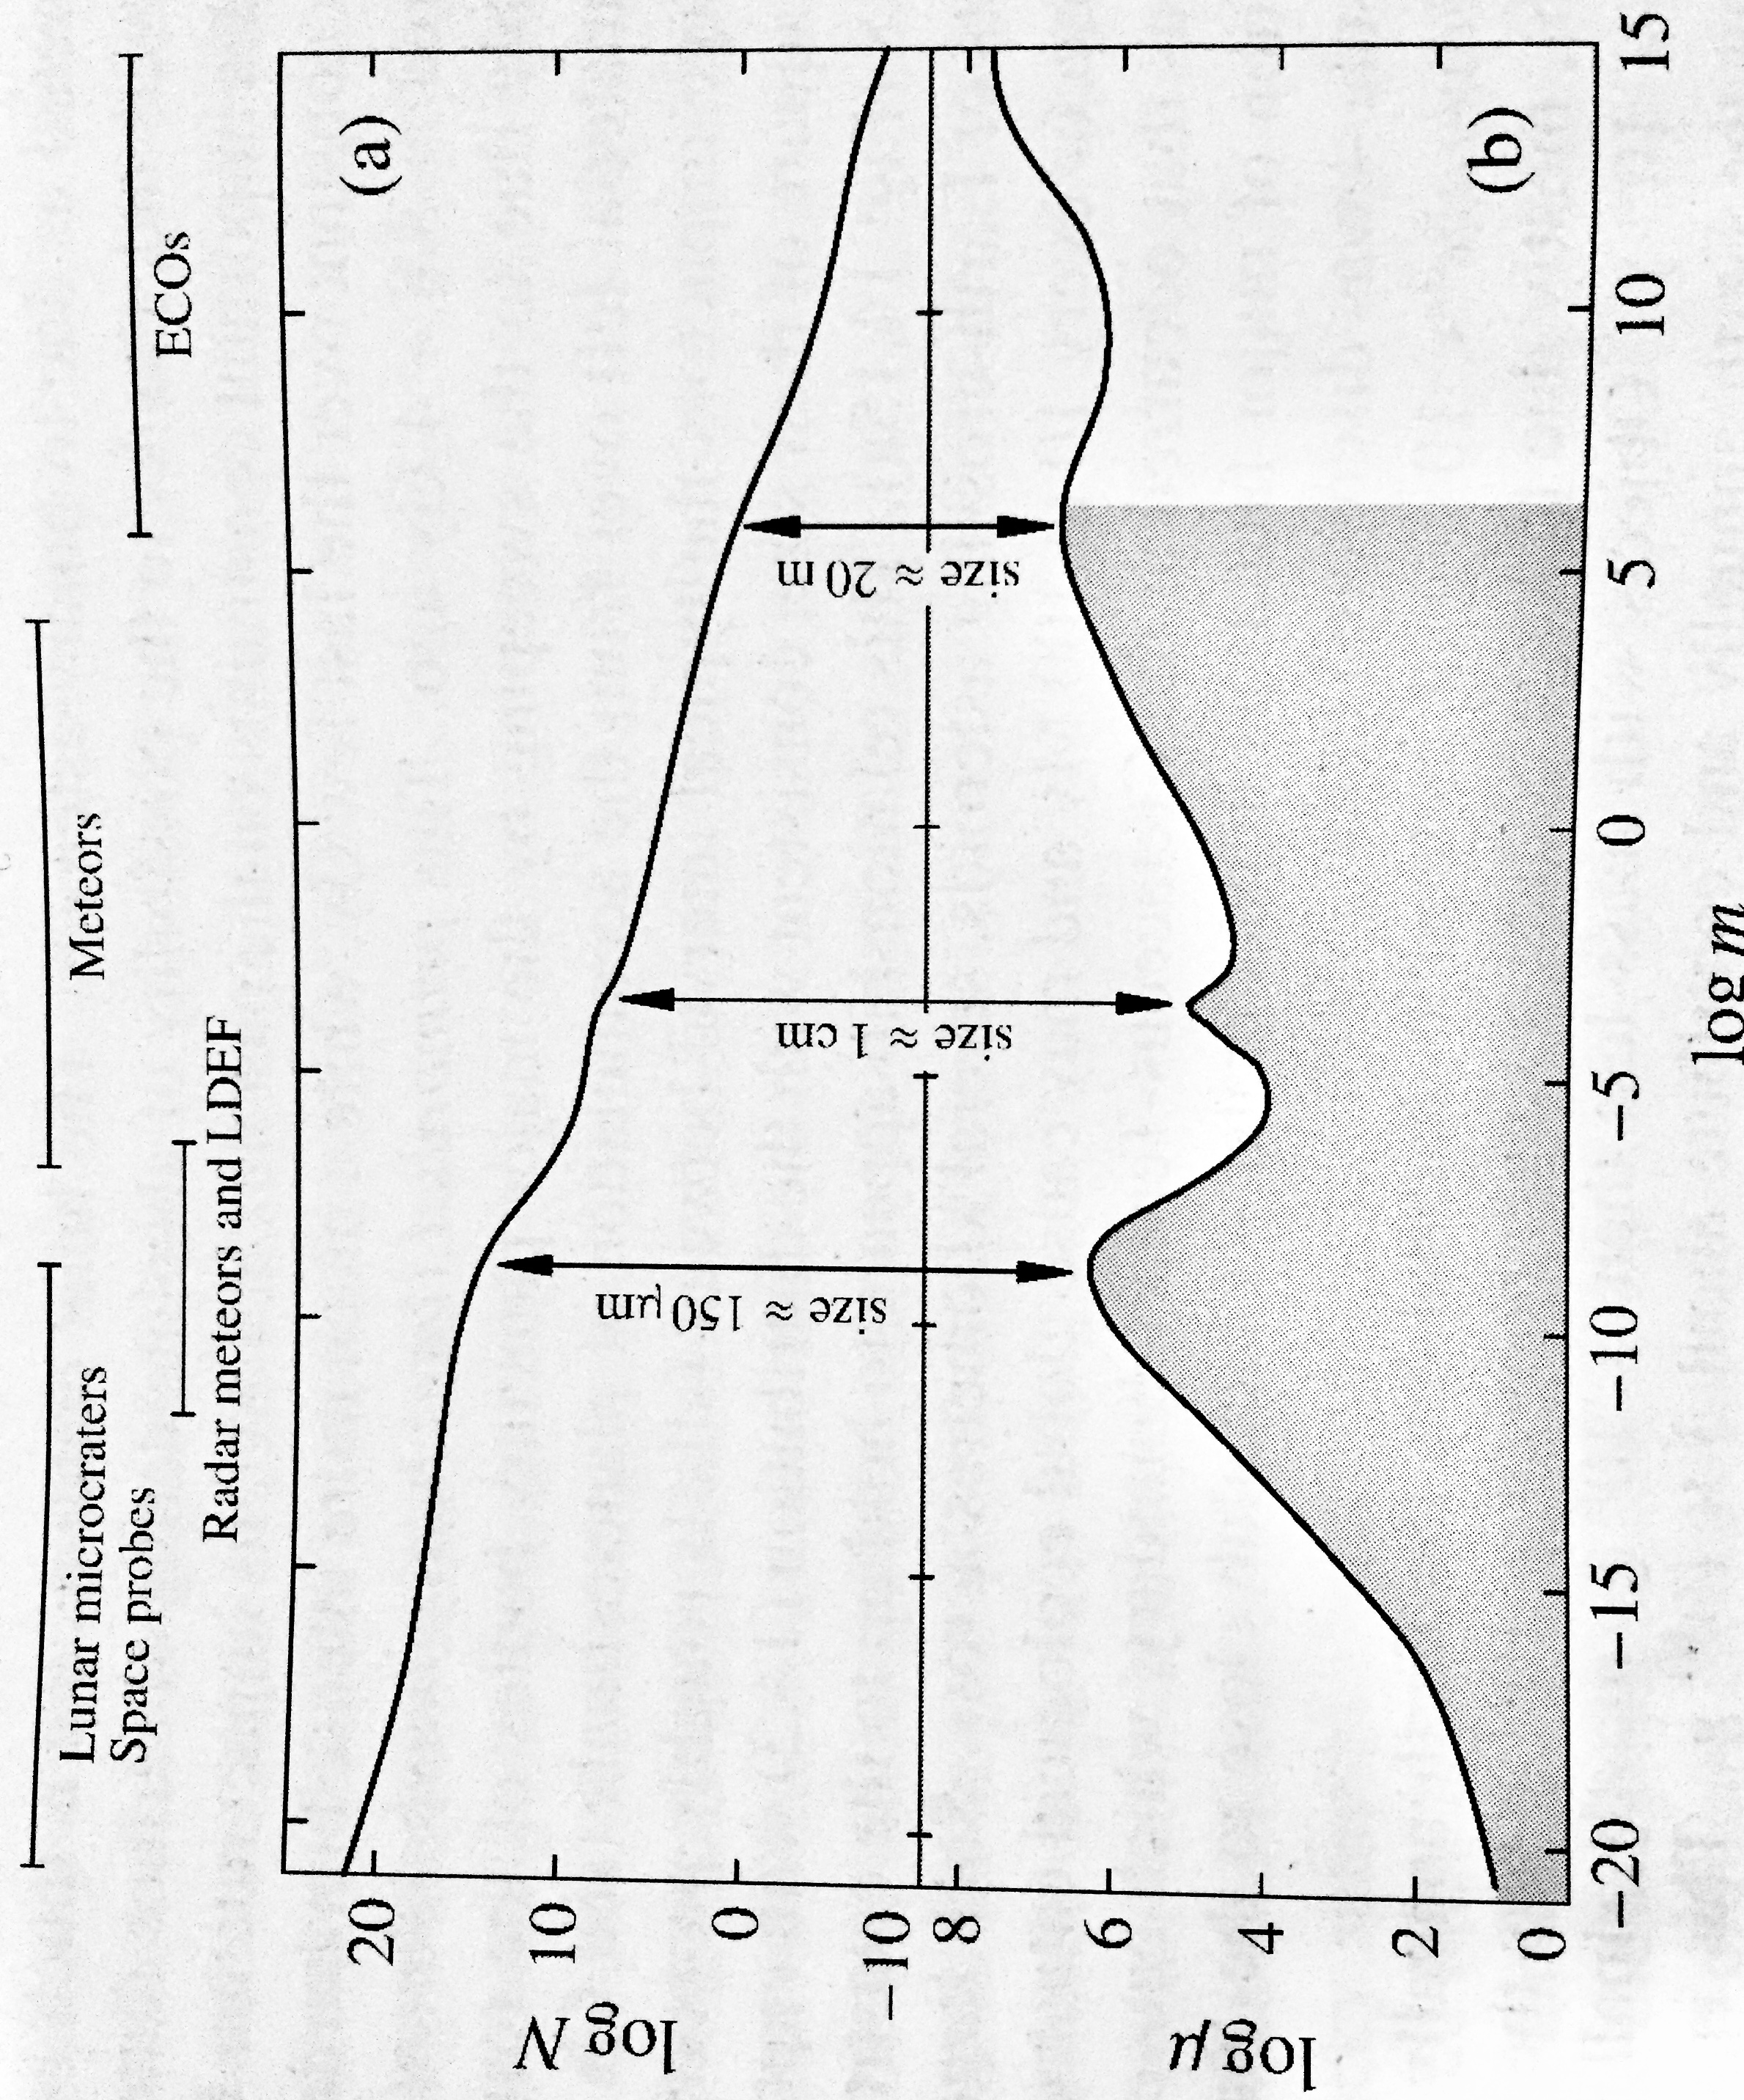
\includegraphics[angle=-90,keepaspectratio,width=\textwidth]{meteorites}\end{figure}
\begin{itemize}
\item Dust band at $I=\pm\deg{2},\pm\deg{10}$ (Inclination of 3 most populated A. families)
\end{itemize}
\begin{block}{Timescale}
\begin{itemize}
\item Crystallization age
\item Cosmic ray exposure age
\item Terrestrial age
\end{itemize}
\end{block}
\end{frame}

\begin{wordonframe}{meteoriti}
$N(m)$ numero oggetti con massa minore di m e $\mu(m)$ is total mass of those object.
\end{wordonframe}

\subsection{Satelliti e anelli}

\begin{frame}{Modello di anello freddo}
\begin{align*}
&m_r=2\pi\rho H\delta r(r_0+\delta r/2)\\
&L=\int\,dm\sqrt{GM_p}r\expy{1/2}=\sqrt{GM_p}2\pi\rho H\int r\expy{3/2}\,dr\\
&E=-\frac{1}{2}GM_p\int \frac{dm}{r}=GM_p\pi\rho H \delta r
\end{align*}
Concentro tutta la massa a una distanza data. Conservazione energia determina un raggio $R_E$, conservazione momento angolare $R_L$:
\begin{align*}
&\frac{R_L}{R_E}\approx1+(\frac{\delta r}{4r_0})^2\\
&\Delta E\approx -\frac{GM_p_r}{r}[(\frac{\delta r}{4r})^2_f-(\frac{\delta r}{4r})^2_i]\approx\frac{GM_p_r}{r}(\frac{\delta r}{4r})^2_i\\
&\Delta E_{grav}\approx\frac{Gm_r^2}{r}
\end{align*}
Per stringer l'anello: $\Delta E_{grav}\geq\Delta E$ cio\'e $\frac{m_r}{M_p}\geq(\frac{\delta r}{4r})^2$.
Un anello stretto: giovane o massiccio o tenuto stretto da altro effetto.
\end{frame}

\begin{wordonframe}{Anello dominato da evoluzione collisionale - freddo - sottile}
Teorema viriale: $\exv{E}=\frac{1}{2}\exv{U}$.
\end{wordonframe}



\subsection{Kuiper, TNO, comete.}\linkdest{Ktnocs}

\begin{frame}{Reservoir di corpi}

\end{frame}

\begin{wordonframe}{Jupiter class comets}

\end{wordonframe}

\begin{frame}{Resonanze in TNO}
The orbits of Pluto and the plutinos are stable, despite crossing that of the much larger Neptune, because they are in a 2:3 resonance with it.
In the rings of Saturn, the Cassini Division is a gap between the inner B Ring and the outer A Ring that has been cleared by a $2:1$ resonance with the moon Mimas. (More specifically, the site of the resonance is the Huygens Gap, which bounds the outer edge of the B Ring.)
    In the rings of Saturn, the Encke and Keeler gaps within the A Ring are cleared by 1:1 resonances with the embedded moonlets Pan and Daphnis, respectively. The A Ring's outer edge is maintained by a destabilizing $7:6$ resonance with the moon Janus.
Most bodies that are in resonance orbit in the same direction; however, a few retrograde damocloids have been found that are temporarily captured in mean-motion resonance with Jupiter or Saturn. Such orbital interactions are weaker than the corresponding interactions between bodies orbiting in the same direction.
\end{frame}

\begin{frame}{Troiani e centauri.}
Troiani: sono oggetti che hanno lo stesso semi-asse di Giove ma spostati di \ang{+-60} nell'orbita cio\'e nei punti Lagrangiani.
Centauri: orbite comprese tra Giove e Nettuno. La zona \'e dinamicamente instabile e porta in orbite cometaria.
\end{frame}

\begin{frame}{Trans-Neptunian object: Fascia di Kuiper-Edgeworth.}
Oltre Nettuno di hanno i TNO.
Un sottogruppo dei TNO, i plutini, sono in risonanza $3:2$ con Nettuno (come Plutone).
\end{frame}

\begin{frame}{Comete}
Orbite eccentriche.

Il cambiamento delle loro propriet\'a dipende dalla distanza dal Sole: ricche di sostanze volatili

Originaria di una fascia esterna di corpi minori compresa tra asteroidi e TNO, in seguito a incontri ravvicinati con corpi maggiori si sono spostate in orbite che raggiungono all'afelio i confini del sistema solare (Nube di Oort approx \SI{e5}{\astronomicalunit}: quando diventa prevalente l'attrazione delle stelle vicine).
\end{frame}

\begin{frame}{Search motivation}
\begin{itemize}
\item Why acretional formation of solar system planet objects should stop at Neptuno's distance.
\item The jupiter family comets are almost on planar orbits with low inclination on ecliptic plane (plane of solar system). This is inesplicable if the source is far away and isotropic, so we may may postulate a a disc of cometary object beyond Neptun.
\end{itemize}
\end{frame}

\subsection{Planetary rings}\linkdest{rings}
